\documentclass{article}

\usepackage{fancyhdr}
\usepackage{extramarks}
\usepackage{amsmath}
\usepackage{amsthm}
\usepackage{amsfonts}
\usepackage{tikz}
\usepackage[plain]{algorithm}
\usepackage{algpseudocode}
\usepackage{graphicx}
\usepackage{gensymb}
\usepackage{calc}
\usepackage[framed,numbered,autolinebreaks,useliterate]{mcode}
\usepackage{listings}
\usepackage{empheq}
\usepackage{enumitem}

\graphicspath{{./images/}}

\usetikzlibrary{automata,positioning}

%
% Basic Document Settings
%

\topmargin=-0.45in
\evensidemargin=0in
\oddsidemargin=0in
\textwidth=6.5in
\textheight=9.0in
\headsep=0.25in

\linespread{1.1}

\pagestyle{fancy}
\lhead{\hmwkAuthorName}
\chead{\hmwkClass\ \hmwkTitle}
\rhead{\firstxmark}
\lfoot{\lastxmark}
\cfoot{\thepage}

\renewcommand\headrulewidth{0.4pt}
\renewcommand\footrulewidth{0.4pt}

\setlength\parindent{0pt}

%
% Create Problem Sections
%

\newcommand{\enterProblemHeader}[1]{
    \nobreak\extramarks{}{Problem {#1} continued on next page\ldots}\nobreak{}
    \nobreak\extramarks{{#1} (continued)}{{#1} continued on next page\ldots}\nobreak{}
}

\newcommand{\exitProblemHeader}[1]{
    \nobreak\extramarks{{#1} (continued)}{{#1} continued on next page\ldots}\nobreak{}
    % \stepcounter{#1}
    \nobreak\extramarks{{#1}}{}\nobreak{}
}

\setcounter{secnumdepth}{0}
\newcounter{partCounter}

\newcommand{\problemNumber}{0.0}

\newenvironment{homeworkProblem}[1][-1]{
    \renewcommand{\problemNumber}{{#1}}
    \section{\problemNumber}
    \setcounter{partCounter}{1}
    \enterProblemHeader{\problemNumber}
}{
    \exitProblemHeader{\problemNumber}
}

%
% Homework Details
%   - Title
%   - Class
%   - Author
%

\newcommand{\hmwkTitle}{Midterm}
\newcommand{\hmwkClass}{RBE 500}
\newcommand{\hmwkAuthorName}{\textbf{Arjan Gupta}}

%
% Title Page
%

\title{
    \vspace{2in}
    \textmd{\textbf{\hmwkClass\ \hmwkTitle}}\\
    \vspace{3in}
}

\author{\hmwkAuthorName}
\date{}

\renewcommand{\part}[1]{\textbf{\large Part \Alph{partCounter}}\stepcounter{partCounter}\\}

%
% Various Helper Commands
%

% Useful for algorithms
\newcommand{\alg}[1]{\textsc{\bfseries \footnotesize #1}}

% For derivatives
\newcommand{\deriv}[2]{\frac{\mathrm{d}}{\mathrm{d}#2} \left(#1\right)}

% For compact derivatives
\newcommand{\derivcomp}[2]{\frac{\mathrm{d}#1}{\mathrm{d}#2}}

% For partial derivatives
\newcommand{\pderiv}[2]{\frac{\partial}{\partial #2} \left(#1\right)}

% For compact partial derivatives
\newcommand{\pderivcomp}[2]{\frac{\partial #1}{\partial #2}}

% Integral dx
\newcommand{\dx}{\mathrm{d}x}

% Alias for the Solution section header
\newcommand{\solution}{\textbf{\large Solution}}

% Probability commands: Expectation, Variance, Covariance, Bias
\newcommand{\E}{\mathrm{E}}
\newcommand{\Var}{\mathrm{Var}}
\newcommand{\Cov}{\mathrm{Cov}}
\newcommand{\Bias}{\mathrm{Bias}}

\newlength\dlf% Define a new measure, dlf
\newcommand\alignedbox[2]{
% Argument #1 = before & if there were no box (lhs)
% Argument #2 = after & if there were no box (rhs)
&  % Alignment sign of the line
{
\settowidth\dlf{$\displaystyle #1$}  
    % The width of \dlf is the width of the lhs, with a displaystyle font
\addtolength\dlf{\fboxsep+\fboxrule}  
    % Add to it the distance to the box, and the width of the line of the box
\hspace{-\dlf}  
    % Move everything dlf units to the left, so that & #1 #2 is aligned under #1 & #2
\boxed{#1 #2}
    % Put a box around lhs and rhs
}
}

\begin{document}

\maketitle

\nobreak\extramarks{Question 1}{}\nobreak{}

\pagebreak

\begin{homeworkProblem}[Question 1]
    Derive the rotation matrix $R^1_2$ (you can leave sines and cosines as is).

    \begin{figure}[h]
        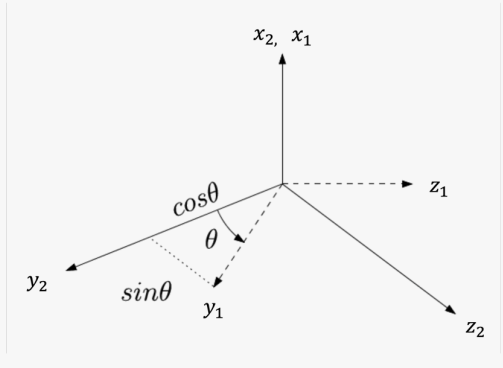
\includegraphics[scale=0.4]{q1_figure.png}
        \centering
    \end{figure}

    \subsection{Solution}

    Since the x-axis remains the same in the rotation, we know this is a basic 3D rotation matrix representing a rotation
    about the x-axis. However, using the right-hand screw rule, we see that the angle $\theta$ here is negative. So, by
    using equation 2.7 (page 43) of our main textbook, the rotation matrix is given by,

    \begin{align*}
        &R^1_2 =
        \begin{bmatrix}
            1 & 0 & 0\\
            0 & \cos(-\theta) & -\sin(-\theta)\\
            0 & \sin(-\theta) & \cos(-\theta)\\
        \end{bmatrix}\\
        \alignedbox{}{R^1_2=
        \begin{bmatrix}
            1 & 0 & 0\\
            0 & \cos\theta & \sin\theta\\
            0 & -\sin\theta & \cos\theta\\
        \end{bmatrix}}
    \end{align*}
\end{homeworkProblem}

\nobreak\extramarks{Question 2}{}\nobreak{}

\pagebreak

\begin{homeworkProblem}[Question 2]
    Find the coordinates of point $p$ expressed in frame 1 (i.e. $p^1$) given the following.

    \[H^2_1 = \begin{bmatrix}
        1 & 0 & 0 & -1\\
        0 & 0.9553 & 0.2955 & -0.9553\\
        0 & -0.2955 & 0.9553 & 0.2955\\
        0 & 0 & 0 & 1
    \end{bmatrix},\text{   } p^2 = \begin{bmatrix}
        2\\
        5\\
        0
    \end{bmatrix}\]

    \subsection{Solution}

    From our knowledge of homogeneous transformations, we know that

    \[P^2 = H^2_1 P^1\]

    Where
    \(P^2 = \begin{bmatrix}
        p^2\\
        1
    \end{bmatrix}\) and \(P^1 = \begin{bmatrix}
        p^1\\
        1
    \end{bmatrix}\).\\

    However, we want to find $P^1$, so we apply the inverse of H to both sides,

    \begin{align*}
        P^2 &= H^2_1 P^1\\
        {(H^2_1)}^{-1}P^2 &= P^1
    \end{align*}

    We know that \(H^2_1 = \begin{bmatrix}
        R^2_1 & d^2_1\\
        0 & 1
    \end{bmatrix}\), where \(R^2_1 = \begin{bmatrix}
        1 & 0 & 0\\
        0 & 0.9553 & 0.2955\\
        0 & -0.2955 & 0.9553
    \end{bmatrix}\) and \(d^2_1 = \begin{bmatrix}
        -1\\
        -0.9553\\
        0.2955
    \end{bmatrix}\).\\
    \vspace{0.15in}\\
    For accuracy while computing the inverse of $H^2_1$, we use equation 2.67 of the book (page 63).
    Therefore, \[{(H^2_1)}^{-1} = \begin{bmatrix}
        {(R^2_1)}^T & -{(R^2_1)}^T d^2_1\\
        0 & 1
    \end{bmatrix}\].
    We use the following MATLAB code for this computation.
    \lstinputlisting{prob2_midterm.m}
    % H2_1 = [1 0 0 -1; 0 0.9553 0.2955 -0.9553; 0 -0.2955 0.9553 0.2955; 0 0 0 1];
    % inv(H2_1)*P2

    Which gives us the answer,

    \[
        \boxed{P^1 = \begin{bmatrix}
            3.0000\\
            5.7764\\
            1.4775\\
            1.0000
        \end{bmatrix}}
    \]
\end{homeworkProblem}

\nobreak\extramarks{Question 3}{}\nobreak{}

\pagebreak

\begin{homeworkProblem}[Question 3]
    If \(R^0_1 = \begin{bmatrix}
        0.7071& 0& 0.7071\\
        0 & 1 & 0\\
        -0.7071& 0& 0.7071
    \end{bmatrix}\), 
    \(R^0_2 = \begin{bmatrix}
        0 & 0.866 & 0.5\\
        0 & 0.5 & -0.866\\
        -1 & 0 & 0
    \end{bmatrix}\), and 
    \(R^0_3 = \begin{bmatrix}
        0 & -1 & 0\\
        0 & 0 & 1\\
        -1 & 0 & 0
    \end{bmatrix}\), calculate $R^1_2$.

    \subsection{Solution}

    Knowing the composition law for rotational transformations, we can write

    \begin{align*}
        R^1_2 &= R^1_0 R^0_2\\
        R^1_2 &= {(R^0_1)}^T R^0_2\\
        R^1_2 &= {\begin{bmatrix}
            0.7071& 0& 0.7071\\
            0 & 1 & 0\\
            -0.7071& 0& 0.7071
        \end{bmatrix}}^T 
        \begin{bmatrix}
            0 & 0.866 & 0.5\\
            0 & 0.5 & -0.866\\
            -1 & 0 & 0
        \end{bmatrix}\\
        R^1_2 &= {\begin{bmatrix}
            0.7071& 0& -0.7071\\
            0 & 1 & 0\\
            0.7071& 0& 0.7071
        \end{bmatrix}} 
        \begin{bmatrix}
            0 & 0.866 & 0.5\\
            0 & 0.5 & -0.866\\
            -1 & 0 & 0
        \end{bmatrix}\\
    \end{align*}

    We use the following MATLAB script to compute this multiplication.
    \lstinputlisting{prob3_midterm.m}

    Therefore,
    \[
        \boxed{
            R^1_2 =
            \begin{bmatrix}
                0.7071 & 0.6123 & 0.3535\\
                0 & 0.5000 & -0.8660\\
               -0.7071 & 0.6123 & 0.3535
            \end{bmatrix}
        }
    \]
\end{homeworkProblem}

\nobreak\extramarks{Question 4}{}\nobreak{}

\pagebreak

\begin{homeworkProblem}[Question 4]

    (a) Calculate Denavit Hertanberg parameters for the given manipulator (just filling out the
    Denavit Hertanberg table would suffice). For this question, you are expected to solve it
    parametrically, i.e.\ you can leave sines, cosines, joint values, and link lengths as
    parameters.

    \begin{figure}[h]
        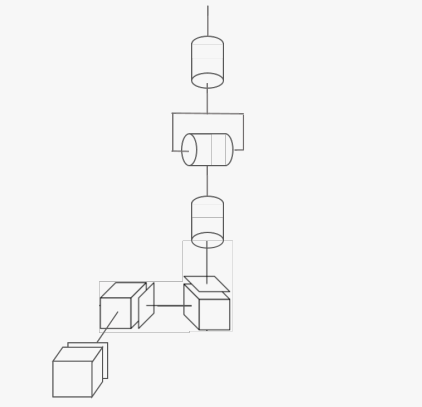
\includegraphics[scale=0.3]{q4_figure.png}
        \centering
    \end{figure}

    (b) Derive $H^1_2$. You can leave sines, cosines, joint values, and link lengths as parameters.
    
    \subsection{Solution for 4(a)}

    First we assign coordinate frames 0 through 5 (links 0 through 5). This is done as per the following figure.

    \begin{figure}[h]
        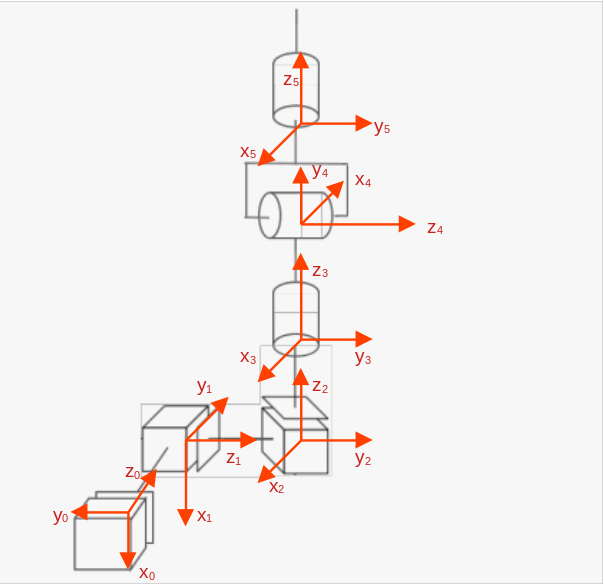
\includegraphics[scale=0.54]{q4_figure_sola.png}
        \centering
    \end{figure}

    Now, we create a table for quantities \(\alpha_i, a_i, \theta_i, d_i\) for links 1 through 6. In this table,
    $d_1$, $d_2$, $d_3$, $\theta_4$, $\theta_5$, $\theta_6$ are variable. However, $l_4$, $l_5$, $l_6$ are fixed (constants).

    \begin{table}[h!]
        \begin{center}
            \begin{tabular}{|c|c|c|c|c|}
            \hline
            Link & $\alpha_i$ & $a_i$ & $\theta_i$ & $d_i$ \\
            \hline
            1 & $90\degree$ & 0 & 0 & $d_1$ \\
            2 & $90\degree$ & 0 & $-90\degree$ & $d_2$\\
            3 & 0 & 0 & 0 & $d_3$\\
            4 & $90\degree$ & 0 & $\theta_4$ & $l_4$\\
            5 & $-90\degree$ & 0 & $\theta_5$ & $l_5$\\
            6 & 0 & 0 & $\theta_6$ & $l_6$\\
            \hline
            \end{tabular}
        \end{center}
    \end{table}

    \subsection{Solution for 4(b)}

    We know that \(H^1_2 = A_2\), where $A_2$ is the DH matrix $A_i$ with $i=2$.
    
    \begin{align*}
        H^1_2 = A_2
        &= \begin{bmatrix}
            \cos\theta_2 & -\sin\theta_2 \cos\alpha_2 & \sin\theta_2 \sin\alpha_2 & a_i \cos\theta_2\\
            \sin\theta_2 & \cos\theta_2 \cos\alpha_2 & -\cos\theta_2 \sin\alpha_2 & a_i \sin\theta_2\\
            0 & \sin\alpha_2 & \cos\alpha_2 & d_2\\
            0 & 0 & 0 & 1
        \end{bmatrix}\\
        &= \begin{bmatrix}
            \cos(-90\degree) & -\sin(-90\degree) \cos(90\degree) & \sin(-90\degree) \sin(90\degree) & a_i \cos(-90\degree)\\
            \sin(-90\degree) & \cos(-90\degree) \cos(90\degree) & -\cos(-90\degree) \sin(90\degree) & a_i \sin(-90\degree)\\
            0 & \sin(90\degree) & \cos(90\degree) & d_2\\
            0 & 0 & 0 & 1
        \end{bmatrix}\\
        \alignedbox{H^1_2}{= \begin{bmatrix}0 & 0 & -1 & 0\\ -1 & 0 & 0 & 0\\ 0 & 1 & 0 & d_{2}\\ 0 & 0 & 0 & 1 \end{bmatrix}}
    \end{align*}

\end{homeworkProblem}

\nobreak\extramarks{Question 5}{}\nobreak{}

\pagebreak

\begin{homeworkProblem}[Question 5]
    Calculate inverse kinematics for the manipulator in Question 4. Assume that all the forward
    kinematics information is available (i.e. all homogenous transformation matrices). Since there
    are no values given, you will be deriving your expressions parametrically, but please be sure to
    explicitly show, which homogeneous transformation matrix is required for the corresponding
    information, and which segment of the matrix is used to obtain that information. (e.g. in your
    derivations you can say something like: “to calculate this expression, I would need $z^0_3$, which is
    available to me at the $3^{rd}$ column of $H^0_3$”).

    \subsection{Solution}

    Before we begin, let us make a brief list of steps we need to take to solve the complete inverse kinematics problem for our 
    particular manipulator's configuration.
    \begin{enumerate}
        \item Find wrist center $o_c$.
        \item Find $q_1$, $q_2$, $q_3$.
        \item Perform forward kinematics to arrive at \(R^0_3 = {(R^3_0)}^T\).
        \item Get \(R^3_6 = R^3_0R^0_6\).
        \item Use $R^3_6$ to find $\phi, \theta, \psi$ of Euler configuration to find $q_4, q_5, q_6$.
    \end{enumerate}
    In essence, once we have found all joint variables given the end-effector's homogeneous transformation, we have solved the inverse kinematics problem.\\

    Now, considering the figure we had in Question 4, let us draw vectors $o_c$ and $o_6$ in it as shown below.

    \begin{figure}[h]
        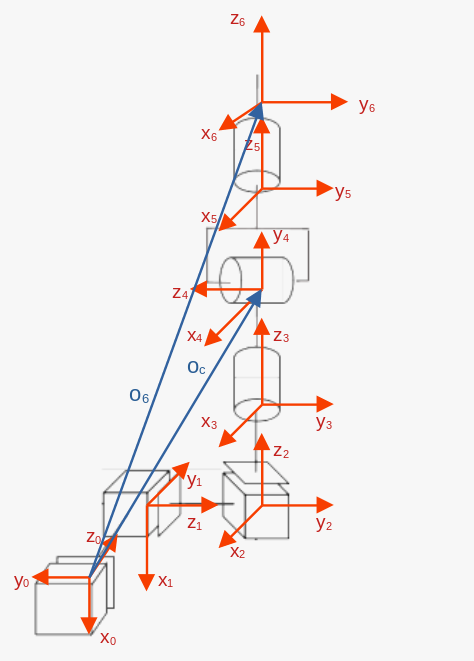
\includegraphics[scale=0.45]{q5_figure_sol.png}
        \centering
    \end{figure}

    We have determined $o_c$ as the wrist center. This is because joints 4, 5, 6 form a spherical wrist, and the z-axes
    of frames 3, 4, 5 intersect at $o_c$. Now let us proceed to Step 1.\\

    \textbf{Step 1} --- Find the wrist center\\

    The end-effector's homogeneous transformation is known to us as the $4\times4$ matrix

    \[
        H^0_6 =
        \begin{bmatrix}
             R^0_6 & o^0_6\\
             0 & 1
        \end{bmatrix}
    \]

    where

    \[
        R^0_6 = 
        \begin{bmatrix}
            r_{11} & r_{12} & r_{13}\\
            r_{21} & r_{22} & r_{23}\\
            r_{31} & r_{32} & r_{33}
        \end{bmatrix},
        o^0_6 =
        \begin{bmatrix}
            x_6 \\
            y_6 \\
            z_6
        \end{bmatrix}
    \]

    Where $o^0_6$ is $o_6$ as shown in the diagram. As shown in the figure, we can establish a relationship between $o_6$ and $o_c$ as

    \[
        \begin{split}
            o_c = o_6 - (l_5 + l_6)R^0_6
            \begin{bmatrix}
                0\\
                0\\
                1
            \end{bmatrix}\\
            \begin{bmatrix}
                x_c \\
                y_c \\
                z_c
            \end{bmatrix}
            =
            \begin{bmatrix}
                x_6 - (l_5 + l_6)r_{13} \\
                y_6 - (l_5 + l_6)r_{23} \\
                z_6 - (l_5 + l_6)r_{33}
            \end{bmatrix}
        \end{split}
    \]

    Where $(l_5 + l_6)$ is a scalar.\\
    
    \textbf{Step 2} --- Find $q_1$, $q_2$, $q_3$.\\

    In the figure we have drawn, we can see that \(x_c = -(d_3 + l_4)\), where $d_3$ is variable and $l_4$ is a constant. Therfore,
    \(d_3 = -x_c - l_4 = -(x_c + l_4)\).\\

    We can also see that \(y_c = -d_2\) and \(z_c = d_1\).\\

    Therefore, we have,
    \begin{empheq}[box=\fbox]{align*}
        q_1 &= d_1 = z_c = z_6 - (l_5 + l_6)r_{33}\\
        q_2 &= d_2 = -y_c = -y_6 + (l_5 + l_6)r_{23}\\
        q_3 &= d_3 = -(x_c + l_4) = -x_6 + (l_5 + l_6)r_{13} - l_4
    \end{empheq}

    \textbf{Step 3} --- Perform forward kinematics\\

    We perform forward kinematics for the first three joint variables. We already found the table in Question 4 as well as $A_2$.
    We write $A_1$ and $A_3$ as the following.
    \[
    A_1 = \begin{bmatrix} 1 & 0 & 0 & 0\\ 0 & 0 & -1 & 0\\ 0 & 1 & 0 & d_{1}\\ 0 & 0 & 0 & 1 \end{bmatrix}
    ,
    A_3 = \begin{bmatrix} 1 & 0 & 0 & 0\\ 0 & 1 & 0 & 0\\ 0 & 0 & 1 & d_{3}\\ 0 & 0 & 0 & 1 \end{bmatrix}
    \]

    We obtain $T^0_3$ using the following MATLAB code.

    \lstinputlisting{./prob5_midterm_fk.m}

    Therefore,
    \[
        T^0_3 =
        \begin{bmatrix} 0 & 0 & -1 & -d_{3}\\ 0 & -1 & 0 & -d_{2}\\ -1 & 0 & 0 & d_{1}\\ 0 & 0 & 0 & 1 \end{bmatrix}
    \]

    From here, it is clear that

    \[
        R^0_3 =
        \begin{bmatrix}
            0 & 0 & -1\\ 0 & -1 & 0\\ -1 & 0 & 0
        \end{bmatrix}
    \]

    \textbf{Step 4} --- Get \(R^3_6 = R^3_0R^0_6\)\\

    We know that $R^3_0 = {(R^0_3)}^T$. Given this fact, we use the following MATLAB code to calculate $R^3_6$.

    \lstinputlisting{./prob5_midterm_step4.m}

    \[
        R^3_6 =
        \begin{bmatrix} -r_{31} & -r_{32} & -r_{33}\\ -r_{21} & -r_{22} & -r_{23}\\ -r_{11} & -r_{12} & -r_{13} \end{bmatrix}
    \]

    \textbf{Step 5} --- Find $q_4$, $q_5$, $q_6$.

    \vspace{0.15in}
    For the final step, we make use of the Euler angles matrix, where $q_4 = \phi, q_5 = \theta, q_6 = \psi$. The matrix for this, as given in
    the textbook, is

    \[
        R^3_6 =
        \begin{bmatrix}
            c_4c_5c_6 - s_4s_6 & -c_4c_5s_6 - s_4c_6 & c_4s_5\\
            s_4c_5c_6 + c_4s_6 & -s_4c_5s_6 + c_4c_6 & s_4s_5\\
            -s_5c_6 & s_5s_6 & c_5
        \end{bmatrix}
    \]

    Now, if we equate this with our matrix from Step 4, we get the third column as,
    \[
        \begin{split}
            c_4s_5 = -r_{33}\\
            s_4s_5 = -r_{23}\\
            c_5 = -r_{13}
        \end{split}
    \]
    And the third row as,
    \[
        \begin{split}
            -s_5c_6 = -r_{11}\\
            s_5s_6 = -r_{12}\\
            c_5 = -r_{13}
        \end{split}
    \]

    So, finally, using equations 2.29, 2.30, 2.31, and 2.32 of the textbook (page 54),

    \[
        \boxed{q_5 = \theta_5 = Atan2(-r_{13}, \sqrt[]{1 - {(-r_{13})}^2})}\\
    \]
    or
    \[
        \boxed{q_5 = \theta_5 = Atan2(-r_{13}, -\sqrt[]{1 - {(-r_{13})}^2})}\\
    \]

    where $Atan2$ is the two-argument algorithmic arctangent function defined in Appendix A of the textbook.\\

    Also,
    \[
        \begin{split}
            \boxed{q_4 = \theta_4 = Atan2(-r_{33}, -r_{23})} \\
            \boxed{q_6 = \theta_6 = Atan2(r_{11}, -r_{12})}\\
        \end{split}
    \]

\end{homeworkProblem}

\nobreak\extramarks{Question 6}{}\nobreak{}

\pagebreak

\begin{homeworkProblem}[Question 6]
    Calculate Jacobian matrix for the manipulator in Question 4. Assume that all the forward
    kinematics information is available (i.e.\ all homogenous transformation matrices). Since there
    are no values given, you will be deriving your Jacobian matrix parametrically, but please be sure
    to explicitly show which homogeneous transformation matrix is required for the corresponding
    information, and which segment of the matrix is used to obtain that information. (e.g. in your
    derivations you can say something like: “to calculate this expression, I would need $z^0_3$, which is
    available to me at the $3^{rd}$ column of $H^0_3$”).

    \subsection{Solution}

    \begin{figure}[h]
        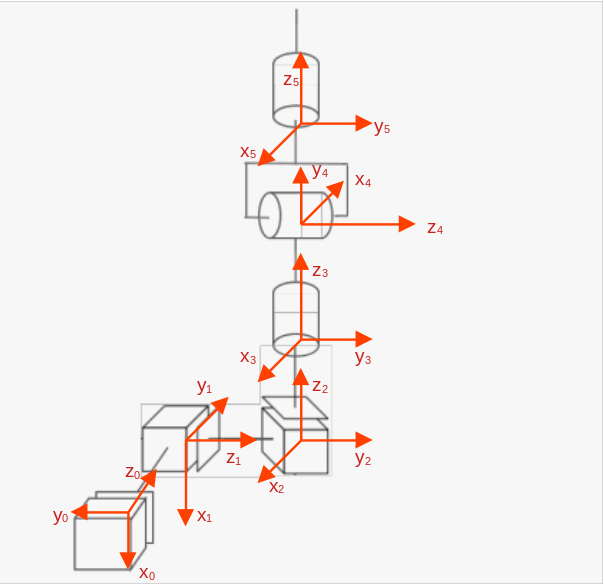
\includegraphics[scale=0.45]{q4_figure_sola.png}
        \centering
    \end{figure}

    \begin{table}[h!]
        \begin{center}
            \begin{tabular}{|c|c|c|}
            \hline
            & Linear component & Angular component\\
            \hline
            Revolute joint & \(J_{v_i} = z^0_{i-1} \times (o^0_n - o^0_{i-1})\) & \(J_{v_i} = z^0_{i-1}\) \\
            Prismatic joint & \(J_{\omega_i} = z^0_{i-1}\) & \(J_{\omega_i} = 0\)\\
            \hline
            \end{tabular}
        \end{center}
    \end{table}
    
    Using this table, and the fact that the upper half of the Jacobian contains linear components while the bottom half
    contains angular components, we have
    \[
        J =
        \begin{bmatrix}
            z_0 & z_1 & z_2 & z_3 \times (o_6 - o_3) & z_4 \times (o_6 - o_4) & z_5 \times (o_6 - o_5) \\
            0 & 0 & 0 & z_3 & z_4 & z_5
        \end{bmatrix}
    \]
\end{homeworkProblem}

\nobreak\extramarks{Question 7}{}\nobreak{}

\pagebreak

\begin{homeworkProblem}[Question 7]
    The dynamic system below
    \[a\ddot{x} + b\dot{x} + c{x} = u\]
    Here u is the force applied to the system, x is the position of the system. $a$, $b$, and $c$ are model
    parameters all of which are constant. There parameters are
     
    \[a = 10, b = 3.5, c = 0.6\]

    \begin{enumerate}[label= (\alph*)]
    \item (5 pts) Find the open loop transfer function for this system, i.e. $\frac{X(s)}{U(s)}$ in laplace domain.
    \item (3 pts) Draw a block diagram of a closed loop system with a PD controller for controlling the position of the system. Explicitly write the transfer functions (Laplace domain) of the system and the PD controller inside the blocks (leave $K_p$ and $K_d$ as parameters).
    \item (5 pts) Derive the closed loop transfer function i.e. $\frac{x}{x_r}$, where $x_r$ is the position reference signal.
    \item (7pts) Find the values of the $K_p$ and $K_d$ gains for a critically damped system with 2 seconds settling time.
    \end{enumerate}
    Show all your steps explicitly.

    \subsection{Solution for 7(a)}

    Transform the system model to Laplace domain on both sides,
    \begin{align*}
        \mathcal{L}\{a\ddot{x} + b\dot{x} + c{x}\} &= \mathcal{L}\{u\}\\
        a X(s) s^2 + b X(s) s + c X(s) &= U(s)\\
    \end{align*}
    \begin{equation}
        X(s)[a s^2 + b s + c] = U(s)
    \end{equation}
    Therefore,
    \[\boxed{\frac{X(s)}{U(s)}=\frac{1}{a s^2 + b s + c}=\frac{1}{10 s^2 + 3.5 s + 0.6}}\]

    \subsection{Solution for 7(b)}

    First let us find the transfer function for the controller. Let our PD controller model be
    \[K_p e + K_d \dot{e} = u\]
    Transform to Laplace domain,
    \begin{align*}
        K_p E(s) + K_d E(s) s &= U(s)\\
        E(s) [K_p + K_d s] &= U(s)
    \end{align*}
    Therefore, the transfer function for the PD controller is
    \begin{equation}
        \frac{U(s)}{E(s)}=K_p + K_d s
    \end{equation}

    Now we can draw the block diagram, as shown on the next page.

    \vspace{3in}

    \begin{figure}
        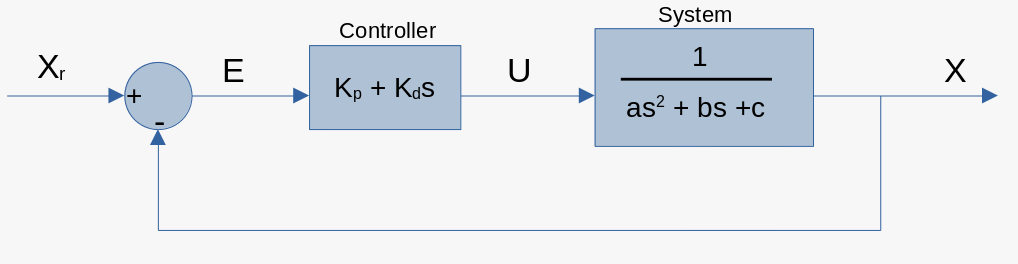
\includegraphics[scale=0.4]{q7_figure.png}
        \centering
    \end{figure}

    \subsection{Solution for 7(c)}
    
    From the block diagram, we can see that
    \[E = X_r - X\]

    Using equation 2 from part (b),

    \[\frac{U(s)}{K_p + K_d s} = X_r - X\]

    Furthermore, using equation 1 from part (a),

    \begin{align*}
        \frac{X(s)[a s^2 + b s + c]}{K_p + K_d s} &= X_r - X\\
        \frac{X [a s^2 + b s + c]}{K_p + K_d s} + X &= X_r\\
        X\left(\frac{a s^2 + b s + c}{K_p + K_d s} + 1\right) &= X_r\\
        X\left(\frac{a s^2 + b s + c + K_p + K_d s}{K_p + K_d s}\right) &= X_r\\
    \end{align*}
    Therefore,
    \[
        \boxed{\frac{X}{X_r}=\frac{K_p + K_d s}{a s^2 + s(b + K_d) + (c + K_p)}=\frac{K_p + K_d s}{10 s^2 + s(3.5 + K_d) + (0.6 + K_p)}}
    \]

    \subsection{Solution for 7(d)}

    Taking the denominator of $\frac{X}{X_r}$, we have the charateristic equation,

    \begin{align*}
        10 s^2 + s(3.5 + K_d) + (0.6 + K_p) &= 0\\
        s^2 + s\frac{3.5 + K_d}{10} + \frac{0.6 + K_p}{10} &= 0
    \end{align*}

    The general form of the charateristic equation is

    \[s^2 + (2\xi\omega_n)s + {\omega_n}^2 = 0\]

    Where $\xi$ is the damping ratio and $\omega_n$ is the natural frequency.\\
    \vspace*{0.3in}\\
    Hence, we have,
    \begin{equation}
        {\omega_n}^2 = \frac{0.6 + K_p}{10}
    \end{equation}
    and
    \begin{equation}
        2\xi\omega_n = \frac{3.5 + K_d}{10}
    \end{equation}

    Also, we know that the natural frequency and settling time $T_s$ are related by

    \[\xi\omega_n T_s = 4\]

    Since we are solving for a critically damped system, we set \(\xi = 1\). We also want settling time $T_s$ = 2 seconds.\\
    
    So, \begin{align*}
        \xi\omega_n T_s &= 4\\
        1 \cdot \omega_n \cdot 2 &= 4\\
        \omega_n &= 2
    \end{align*}

    Plugging this into equation 3, we have

    \begin{align*}
        {(2)}^2 &= \frac{0.6 + K_p}{10}\\
        40 &= 0.6 + K_p\\
        \alignedbox{K_p}{=39.4}
    \end{align*}

    Also, plugging in values into equation 4, we have

    \begin{align*}
        2(1)(2) &= \frac{3.5 + K_d}{10}\\
        40 &= 3.5 + K_d\\
        \alignedbox{K_d}{=36.5}
    \end{align*}
\end{homeworkProblem}

\nobreak\extramarks{Question 8}{}\nobreak{}

\pagebreak

\begin{homeworkProblem}[Question 8]
    
\end{homeworkProblem}

\end{document}